\documentclass{article}
\usepackage{listings}
\usepackage{amsmath}
\usepackage{fancyhdr}
\usepackage{draftwatermark}
\usepackage {sectsty}
\usepackage{hyperref}
\usepackage{graphicx}
\graphicspath{ {img/} }
\usepackage [dvipsnames]{xcolor}

\lstset{ %
	language=C,
	basicstyle=\ttfamily\footnotesize,
	keywordstyle=\ttfamily\color{blue}\footnotesize,
	commentstyle=\color{OliveGreen}\ttfamily\footnotesize,
	texcl,
	escapechar =`
	escapebegin=\lst@commentstyle,
	showspaces=false,
	showtabs=false,
	numbers=left,
	showstringspaces=false,
	frame=single,
	tabsize=3
}
\makeatother


\pagestyle{fancy}
\renewcommand{\rightmark}{}

\SetWatermarkText{DRAFT}
\SetWatermarkScale{5}
\SetWatermarkLightness{.98}

\sectionfont{\color{cyan}}
\author{Sean Curran \\
\and Stephen Durofchalk \\
\and Zachary Feldman \\
\and Ryan Wails}
\title{CMPEN/EE 454 Project 2 Report}

\begin{document}

\maketitle
\thispagestyle{empty}

\newpage
\pagenumbering{roman}
\setcounter{page}{1}
\setcounter{tocdepth}{2}
\tableofcontents
\thispagestyle{plain}

\newpage
\pagenumbering{arabic}
\setcounter{page}{1}
\section{Integral Algorithms}
\subsection{Harris Corner Detection}
\subsubsection{Synopsis}
Harris corner detection is an algorithm which detect corners in images that can be used to create point correspondences between time series images.  A ``corner'' can loosely be defined as a feature in the image located at coordinates $(x_0,y_0)$ such that $\frac{\partial I}{\partial x}(x_0,y_0)$ and $\frac{\partial I}{\partial y}(x_0,y_0)$ yield relatively large values.
\subsubsection{Implementation}
Below the implementation of the Harris corner detection algorithm in C-like pseudocode.
\begin{lstlisting}

intensity_image harris(original_image, patch_indices) {

	// Compute the image patch.
	intensity_img = convert_to_intensity_image(original_image);
	img_patch = compute_patch(intensity_img, patch_indices);
	
	// Compute partial x and y, mixed derivatives.
	ix = convolve_sobel_x(img_patch);
	iy = convolve_sobel_y(img_patch);
	
	ix2 = ix * ix;
	iy2 = iy * iy;
	ixy = ix * iy;

	// Compute sums using a Gaussian windowing function
	sx2 = convolve_gaussian(ix2);
	sy2 = convolve_gaussian(iy2);
	sxy = convolve_gaussian(ixy);
	
	// For each pixel in the image, compute H matrix,
	// compute product of eigenvalues scaled by k = 0.07,
	// and store the response value as r.
	for (px : img_patch) {
		H = {{sx2(px), sxy(px)}, {sxy(px) sy2(px)}};
		r(px) = det(H) - 0.07 * trace(H) * trace(H);
	}
	
	return r;
}

\end{lstlisting}
This routine returns a non-normalized intensity image where strong intensities correspond to corner points in the image patch.  Once this intensity image has been computed, it is passed to a thresholding routine where the coordinate points of these corners is determined.

\begin{minipage}{\textwidth}
\begin{lstlisting}

pixel_array compute_coordinates(intensity_image, threshold) {

	// First, we optionally use a monte-carlo pruning algorithm
	// to reduce the number of corner coordinated produced by this
	// function.
	prune(intensity_image);

	// Next, the intensity image is converted to a binary image.
	b_img = threshold_to_binary(intensity_image, threshold);
	
	// Finally, any pixel with a value of 1 in the binary image
	// is considered a corner point coordinate.
	// 
	// The notation for(x:y) is used to mean "for each element x
	// in the set y."
	for (px : b_img) {
		p_array.add(px);
	}
	
	return p_array;
}

\end{lstlisting}
\end{minipage}

\newpage
\subsection{Patch Matching}
\subsubsection{Synopsis}
After the corner point coordinates of each image has been computed, the bounding boxes for each image and corresponding corner points are passed to a patch matching routine.  This patch matching routine computes correspondences between corner points and between bounding boxes (explained in more detail below).  The in the system pictured below, assuming the image in bounding boxes 1 and 3 are similar and the images in bounding boxes 2 and 4 are similar, the correspondence set output for this phase would be:
\[
\left \{
\begin{tabular}{c}
$(1 \iff 3,\quad \text{assignment cost})$ \\
$(2 \iff 4,\quad \text{assignment cost})$
\end{tabular}
\right \}
\]
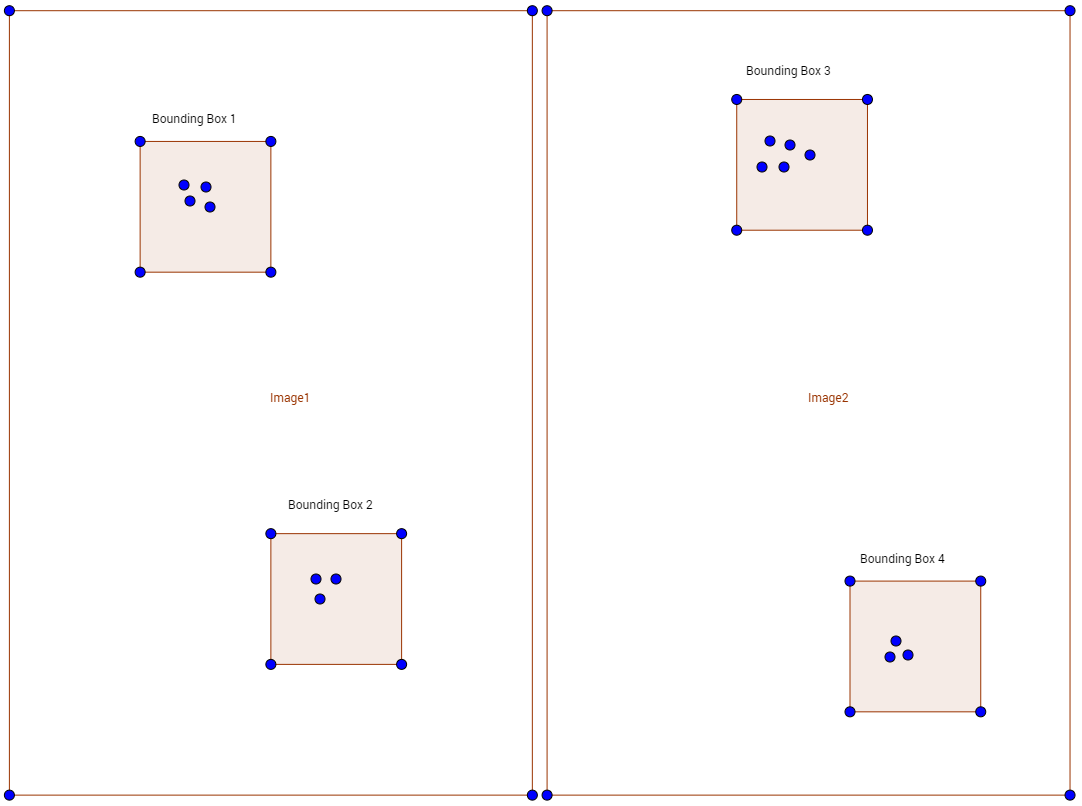
\includegraphics[width=\textwidth]{after_corner}
\subsubsection{Implementation}
To find an optimal bounding box correspondence set between two images, we first must compute cost values for matching two boxes.  Here is the implemented cost function:
\\
\begin{minipage}{\textwidth}
\begin{lstlisting}

assignment_set compute_bb_set(bounding_box_a, bounding_box_b) {

	// Compute the costs of corresponding each corner
	// point in bounding box a against every corner
	// point in bounding box b.
	for (corner_a : bounding_box_a) {
	for (corner_b : bounding_box_b) {
		// Get the image patches around each corner point.
		patch_a = get_patch(corner_a);
		patch_b = get_patch(corner_b);
			
		// Use SSD as cost function.
		cost_matrix[corner_a, corner_b] =
			sum_squared_difference(patch_a, patch_b);
	} }
	
	// Use the provided optimal assingment algorithm to get
	// a point correspondence set and the costs assiociated
	// with each assignment.
	return assignmentoptimal(cost_matrix);
}

\end{lstlisting}
\end{minipage}
\\~\\
For the bounding boxes pictured below, here is an example assignment set:
\[
\left \{
\begin{tabular}{c}
$(G \iff J,\quad \text{SSD}_{GJ})$ \\
$(F \iff K,\quad \text{SSD}_{FK})$ \\
$(I \iff M,\quad \text{SSD}_{IM})$ \\
$(E \iff \emptyset,\quad \infty)$ \\
$(H \iff \emptyset,\quad \infty)$
\end{tabular}
\right \}
\]
The overall cost of assigning Bounding Box 1 to Bounding Box 2 is then the sum of the finite costs in the optimal assignment set; i.e. $\text{SSD}_{GJ} + \text{SSD}_{FK} + \text{SSD}_{IM}$.
\begin{center}
\fbox{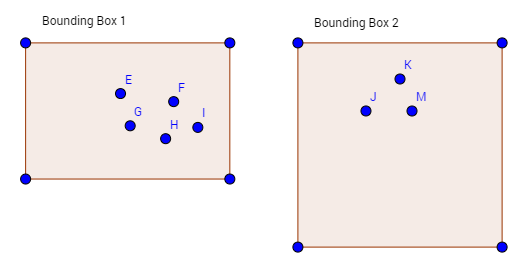
\includegraphics[width=0.65\textwidth]{box_corners}}
\end{center}
~\\
A similar method is used to find an optimal bounding box correspondence between two images:
\\
\begin{minipage}{\textwidth}
\begin{lstlisting}

assignment_set compute_img_set(image_a, image_b) {

	// Compute the costs of corresponding each bounding box
	// in image a against every bounding box in image b.
	for (bounding_box_a : image_a) {
	for (bounding_box_b : image_b) {
		
		bb_set =
		compute_bb_set(bounding_box_a, bounding_box_b);
		
		// Sum the costs for the valid assignments
		total_cost = 0;
		for (assignment : bb_set) 
			if (assignment.cost < inf)
				total_cost += assignment.cost;
		
		cost_matrix[bounding_box_a, bounding_box_b] =
			total_cost;
		
	} }
	
	return assignmentoptimal(cost_matrix);
}

\end{lstlisting}
\end{minipage}
\newpage
\subsection{RANSAC}
\subsubsection{Synopsis}
Once the optimal bounding box correspondences have been determined, random sample consensus (RANSAC) can be used to estimate the translation of a bounding box between two images.  RANSAC is a probabilistic, consensus-based algorithm which can be used to efficiently remove outliers from a set - in this problem space, outliers are ``bad'' corner points correspondences determined by the \texttt{compute\_bb\_set} function.
\subsubsection{Implementation}
\begin{minipage}{\textwidth}
\begin{lstlisting}

estimated_translation ransac(bounding_box_i, bounding_box_j,
	num_iterations, threshold) {

// Perform the inner-routine num\_iteartion times.
for (i = 1 to num_iterations) {
	// Get a random pair of corresponding corners
	// from the bounding boxes.
	corner_i = get_random_corner(bounding_box_i);
	corner_j =
	get_corresponding_corner(bounding_box_j, corner_i);
	
	// Get the component-wise translation between these
	// corresponding points.
	translation = compute_translation(corner_i, corner_j);
	
	inlier_count = 0;
	max_inlier_count = 0, best_translation = 0;
	
	for (corner : bounding_box_i) {
		// Estimate where all the other corners should be based
		// on the translation computed above.
		estimated_corner = corner + translation;
		
		// Get the actual correspondence point
		actual_corner =
			get_corresponding_corner(bounding_box_j, corner);
		
		// If the estimated point is close to the actual point,
		// consider the point an inlier.
		distance = l2norm(actual_corner, estimated_corner);
		if (distance < threshold) inlier_count++;
	}
	
	// Keep track of the best translation estimate.
	if (inlier_count > max_inlier_count) {
		max_inlier_count = inlier_count;
		best_translation = translation;
	}
		
} return best_translation; }

\end{lstlisting}
\end{minipage}

\end{document}